\documentclass{beamer}

\usetheme{focus} % Use the Focus theme supplied with the template
% Add option [numbering=none] to disable the footer progress bar
% Add option [numbering=fullbar] to show the footer progress bar as always full with a slide count
\usepackage{tikz}
\usepackage{amsmath}
\usepackage{setspace}
\usepackage[most]{tcolorbox}
\usetikzlibrary{fadings,decorations.markings,arrows,shapes}
\tcbuselibrary{skins}
\newtcolorbox{mybluebox}[2][]{%
    colback=bg, 
    colframe=blue!75!black,
    fonttitle=\bfseries,
    coltitle=blue!75!black, 
    colbacktitle=bg,
    enhanced,
    attach boxed title to top left={yshift=-1.2mm, xshift=2mm},
  title=#2,
  #1}   


% Uncomment to enable the ice-blue theme
%\definecolor{main}{RGB}{92, 138, 168}
%\definecolor{background}{RGB}{240, 247, 255}

%------------------------------------------------

\usepackage{booktabs} % Required for better table rules

%----------------------------------------------------------------------------------------
%	 TITLE SLIDE
%----------------------------------------------------------------------------------------

\title{Overrepresetation: \\ Algorithms for Gene Ontology}

\subtitle{From Fisher to Bayes}

\author{Peter N Robinson}

\titlegraphic{
\includegraphics[scale=0.75]{img/JGMlogo.png}} % Optional title page image, comment this line to remove it

\institute{The Jackson Laboratory \\ Farmington CT}

\date{2022-10-??}

%------------------------------------------------

\begin{document}

%------------------------------------------------

\begin{frame}
	\maketitle % Automatically created using the information in the commands above
\end{frame}

%----------------------------------------------------------------------------------------
%	 SECTION 1
%----------------------------------------------------------------------------------------

\section{Gene Ontology} % Section title slide, unnumbered

%------------------------------------------------

%%%%%%%%%%%%%%%%%%%%%%%%%%%%%%%%%%%%%%%%%%%%%%%%%%%%%%%%%%%%%%%%%%%
%%%%%%%%%%%%%%%%%%%%%%%%%%%%%%%%%%%%%%%%%%%%%%%%%%%%%%%%%%%%%%%%%%%
\begin{frame}{Gene Ontology}
    \begin{mybluebox}{Gene Ontology (GO)}
    GO is being developed with the goal of providing a
    set of structured vocabularies for the annotation of genes and their products. Since    	the publication  of the original paper in \emph{Nature Genetics} in 2000, GO
    has become one of the most widely used and mature bio-ontologies,
    although it is still very much a work in progress~\cite{GO2019}.
    \end{mybluebox}
    
    \begin{figure}
     \centering
     
\includegraphics[width=0.25\textwidth]{./img/GOlogo.png}
    \end{figure}
    
\end{frame}

%------------------------------------------------

%%%%%%%
%%%%%%%%%%%%%%%%%%%%%%%%%%%%%%%%%%%%%%%%%%%%%%%%%%%%%%%%%%%%%%%%%%%%%%%%%%%%%%%%%%%%%%%%%%%%%%%%%%%%
\begin{frame}{Why do we need GO?}
\begin{itemize}
\item Exponential increase in biological data $\longmapsto$ need for databases with appropriate 
representation techniques
\item Progress in the way biologists describe functions has not kept pace with the results of 
large-scale sequencing projects $\longmapsto$ need for eff{}icient high-quality procedures for 
(preliminary) annotation of genes (e.g. \textit{Drosophila} genome)
\item Nomeclature for genes, gene products, and functions is widely divergent between dif{}ferent 
databases $\longmapsto$ too diff{}icult to compare between species

\item Uses: Information extraction, data mining, database integration...

\end{itemize}
\end{frame}

%%%%%%%%%%%%%%%%%%%%%%%%%%%%%%%%%%%%%%%%%%%%%%%
%%%%%%%%%%%%%%%%%%%%%%%%%%%%%%%%%%%%%%%%%%%%%%%

\begin{frame}{What came before GO?}
\begin{mybluebox}{Enzyme Commission}
    Before GO came on the scene, biological functions were represented as trees.
\end{mybluebox}
\vspace{-5mm}

\begin{center}
  \begin{tabular}{cp{5mm}c}
    \rotatebox{270}{ \resizebox{0.3\textheight}{!}{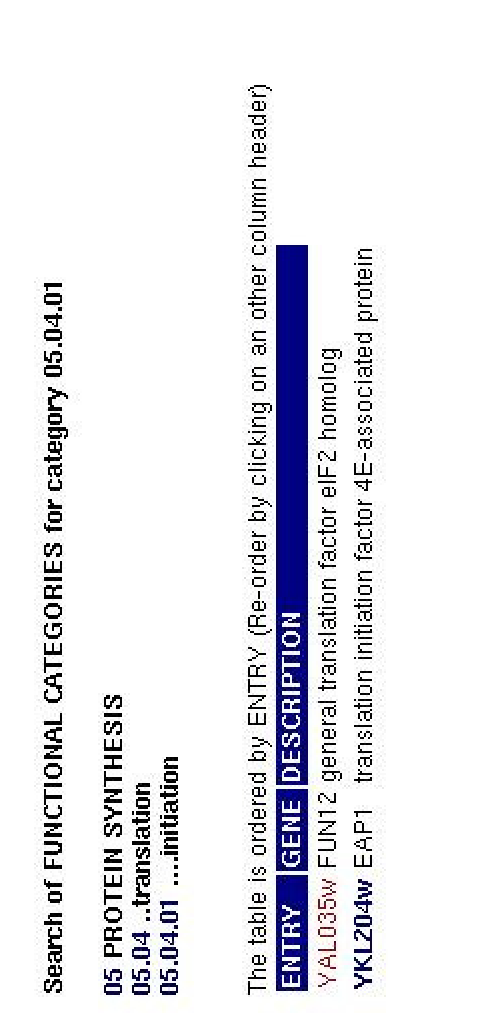
\includegraphics{img/mips.pdf}} }&
	&
     \rotatebox{270}{\resizebox{0.3\textheight}{!}{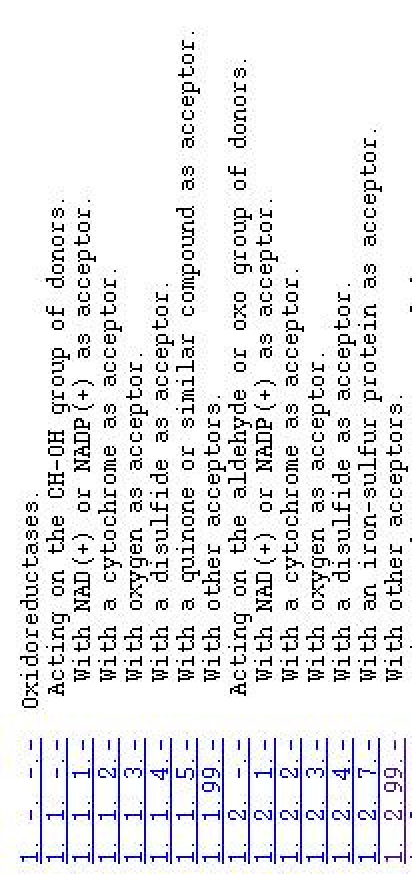
\includegraphics{img/EC.pdf}}} \\
 	MIPS & & EC \\
  \end{tabular}
\end{center}

\begin{itemize}
\item MIPS: Munich Information Center for Protein Sequences
\item EC: Enzyme commision def{}initions of enzyme classes, subclasses and sub-subclasses
\end{itemize} 

\end{frame}

%%%%%%%%%%%%%%%%%%%%%%%%%%%%%%%%%%%%%%%%%%%%%%%
%%%%%%%%%%%%%%%%%%%%%%%%%%%%%%%%%%%%%%%%%%%%%%%

\begin{frame}{Function?}
The term function is sometimes used in a rather vague way..
\begin{itemize}
\item biochemical activity
\item biological goals
\item subcellular localization
\end{itemize} 

\begin{figure}
\centering
\rotatebox{270}{
\resizebox{0.5\textheight}{!}{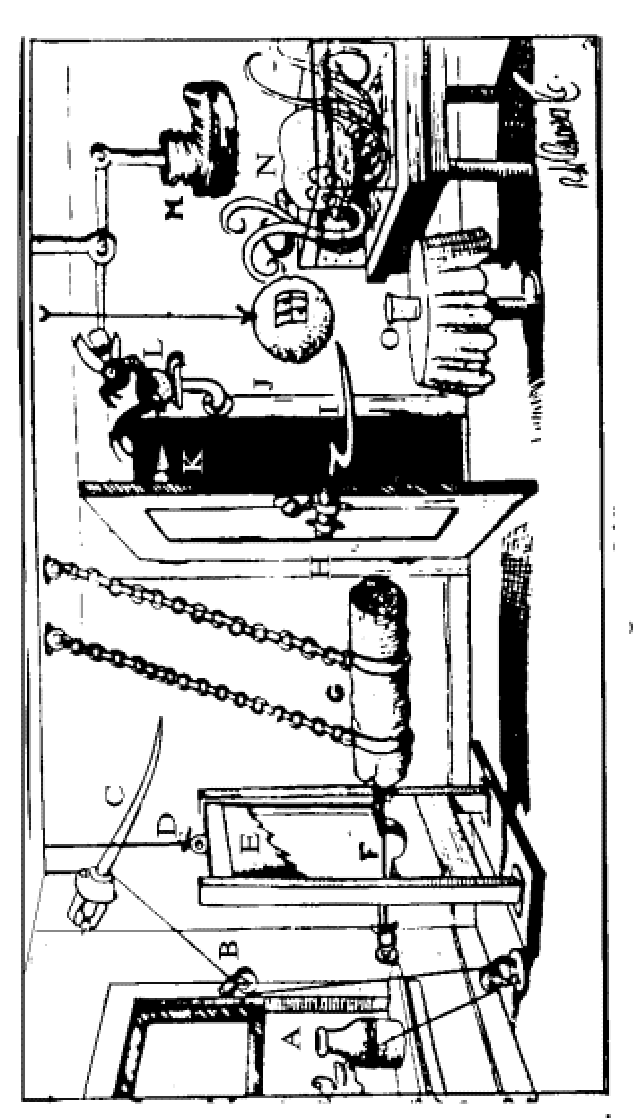
\includegraphics{img/rube.pdf}}
}
\end{figure}

\end{frame}


%%%%%%%%%%%%%%%%%%%%%%%%%%%%%%%%%%%%%%%%%%%%%%%
%%%%%%%%%%%%%%%%%%%%%%%%%%%%%%%%%%%%%%%%%%%%%%%

\begin{frame}{GO: Biological Process}
\begin{itemize}
\item Biological objective to which the gene or gene product contributes
\item A process is accomplished by one or more assemblies of molecular functions
\item Often involve chemical or physical transformation
\item Examples: (High level) \textquotedblleft Signal Transduction\textquotedblright, 
\textquotedblleft Cell Growth and Maintenance\textquotedblright
\item Examples: (Lower level) \textquotedblleft pyrimidine metabolism\textquotedblright, 
\textquotedblleft cAMP biosynthesis\textquotedblright
\end{itemize}
\end{frame}

%%%%%%%%%%%%%%%%%%%%%%%%%%%%%%%%%%%%%%%%%%%%%%%
%%%%%%%%%%%%%%%%%%%%%%%%%%%%%%%%%%%%%%%%%%%%%%%

\begin{frame}{GO: Biological Process (2)}
\begin{center}
\rotatebox{270}{
\resizebox*{!}{1\textheight}{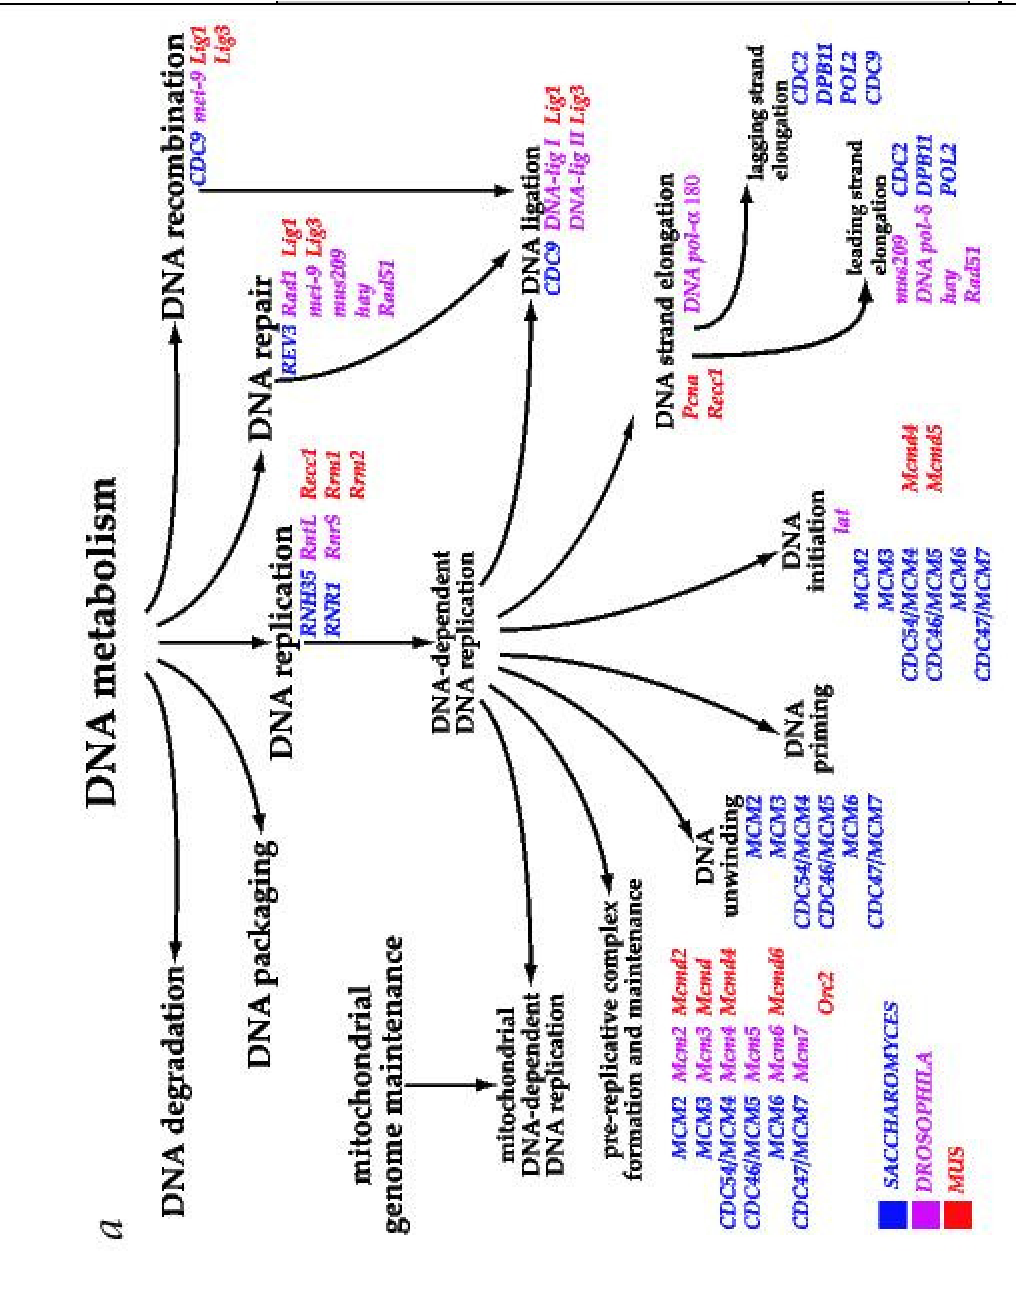
\includegraphics{img/dnametabolism.pdf}}
}
\end{center}
\end{frame}

%%%%%%%%%%%%%%%%%%%%%%%%%%%%%%%%%%%%%%%%%%%%%%%
%%%%%%%%%%%%%%%%%%%%%%%%%%%%%%%%%%%%%%%%%%%%%%%

\begin{frame}{GO: Molecular Function}
\begin{itemize}
\item Biochemical activity of a gene product
\item describes \textit{what} is done rather than why or where or when
\item Examples: (High level) \textquotedblleft Enzyme',  \textquotedblleft 
transporter\textquotedblright
\item Examples: (Lower level) \textquotedblleft adenylate cyclase\textquotedblright, 
\textquotedblleft Toll receptor ligand\textquotedblright
\end{itemize}
\end{frame}
%%%%%%%%%%%%%%%%%%%%%%%%%%%%%%%%%%%%%%%%%%%%%%%
%%%%%%%%%%%%%%%%%%%%%%%%%%%%%%%%%%%%%%%%%%%%%%%
\begin{frame}{GO: Molecular Function (2)}
\begin{center}
\rotatebox{270}{
\resizebox*{!}{1\textheight}{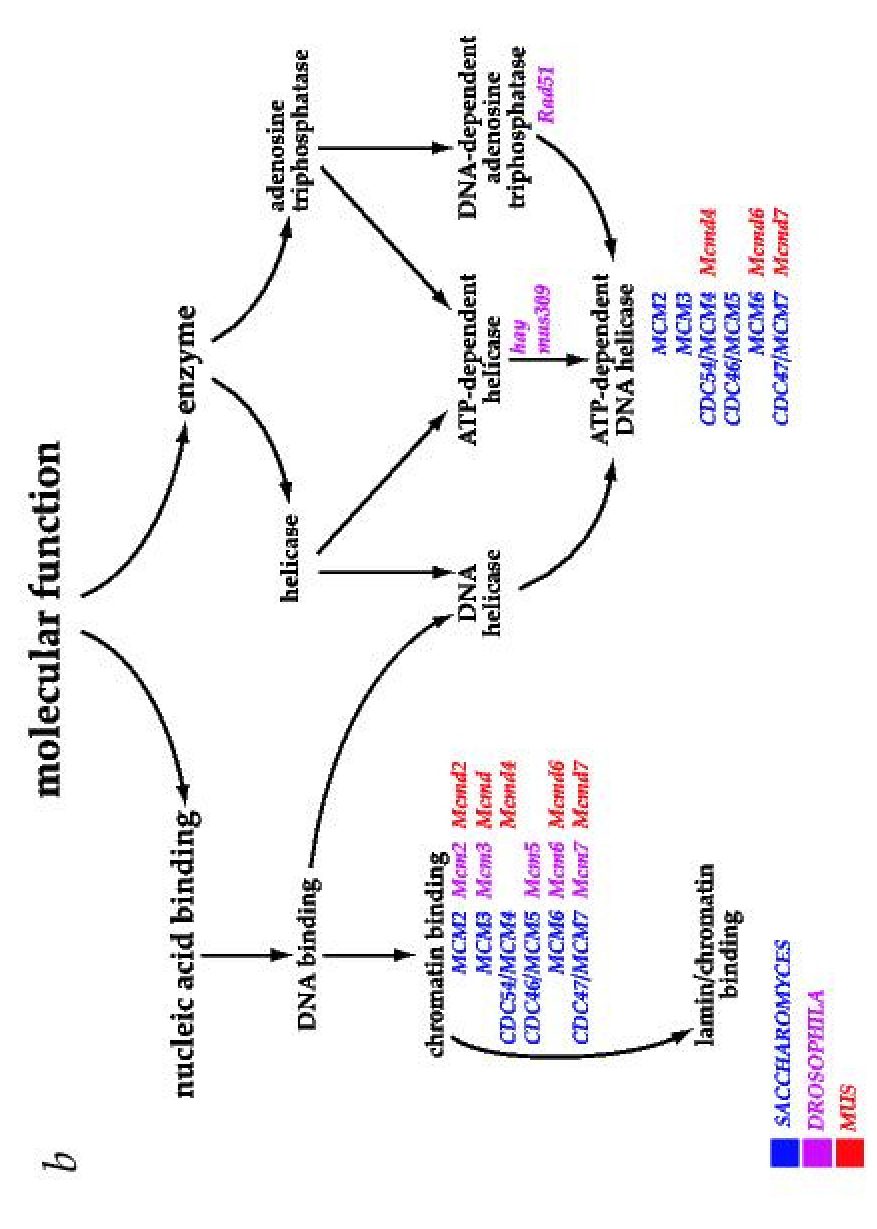
\includegraphics{img/molecularfun.pdf}}
}
\end{center}
\end{frame}

%%%%%%%%%%%%%%%%%%%%%%%%%%%%%%%%%%%%%%%%%%%%%%%
%%%%%%%%%%%%%%%%%%%%%%%%%%%%%%%%%%%%%%%%%%%%%%%
\begin{frame}{GO: Cellular component}
\begin{itemize}
\item Place in the cell where a gene product is active
\item Example: \textquotedblleft Nuclear membrane\textquotedblright
\item Can also refer to entities made up of multiple gene products are to be found
\item Example: \textquotedblleft ribosome\textquotedblright, \textquotedblleft 
proteosome\textquotedblright
\end{itemize}
\end{frame}
%%%%%%%%%%%%%%%%%%%%%%%%%%%%%%%%%%%%%%%%%%%%%%%
%%%%%%%%%%%%%%%%%%%%%%%%%%%%%%%%%%%%%%%%%%%%%%%
\begin{frame}{GO: Cellular component (2)}
\begin{center}
\rotatebox{270}{
\resizebox*{!}{1\textheight}{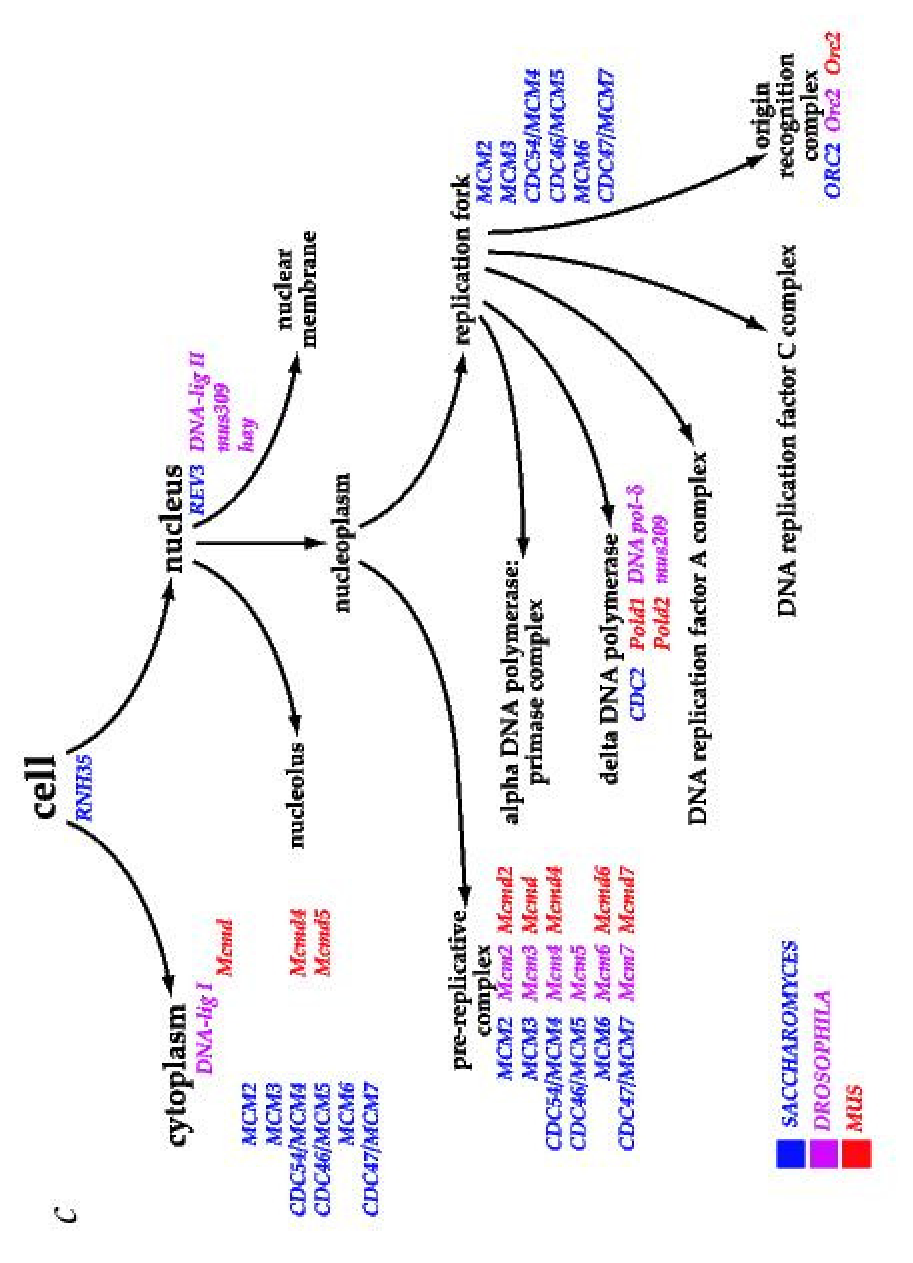
\includegraphics{img/cellcomponent.pdf}}
}
\end{center}
\end{frame}
%%%%%%%%%%%%%%%%%%%%%%%%%%%%%%%%%%%%%%%%%%%%%%%
%%%%%%%%%%%%%%%%%%%%%%%%%%%%%%%%%%%%%%%%%%%%%%%

% GO terms
\begin{frame}{GO Terms}
\begin{itemize}
\item GO:0003678
\item Name: DNA helicase activity
\item Def{}inition: Catalysis of the the hydrolysis of ATP to unwind the DNA helix at the 
replication fork, allowing the resulting single strands to be copied.
\item Information about parent terms (bookkeeping of the DAG structure)
\end{itemize} 
\begin{small}Each entry (\textit{term}) in GO contains this information\end{small}
\end{frame}
%%%%%%%%%%%%%%%%%%%%%%%%%%%%%%%%%%%%%%%%%%%%%%%
%%%%%%%%%%%%%%%%%%%%%%%%%%%%%%%%%%%%%%%%%%%%%%%


\begin{frame}{GO Annotations}
\begin{itemize}
\item Annotations are available for numerous species
\item GO can be regarded as an {\bf attribute ontology}
\end{itemize}
\begin{center}
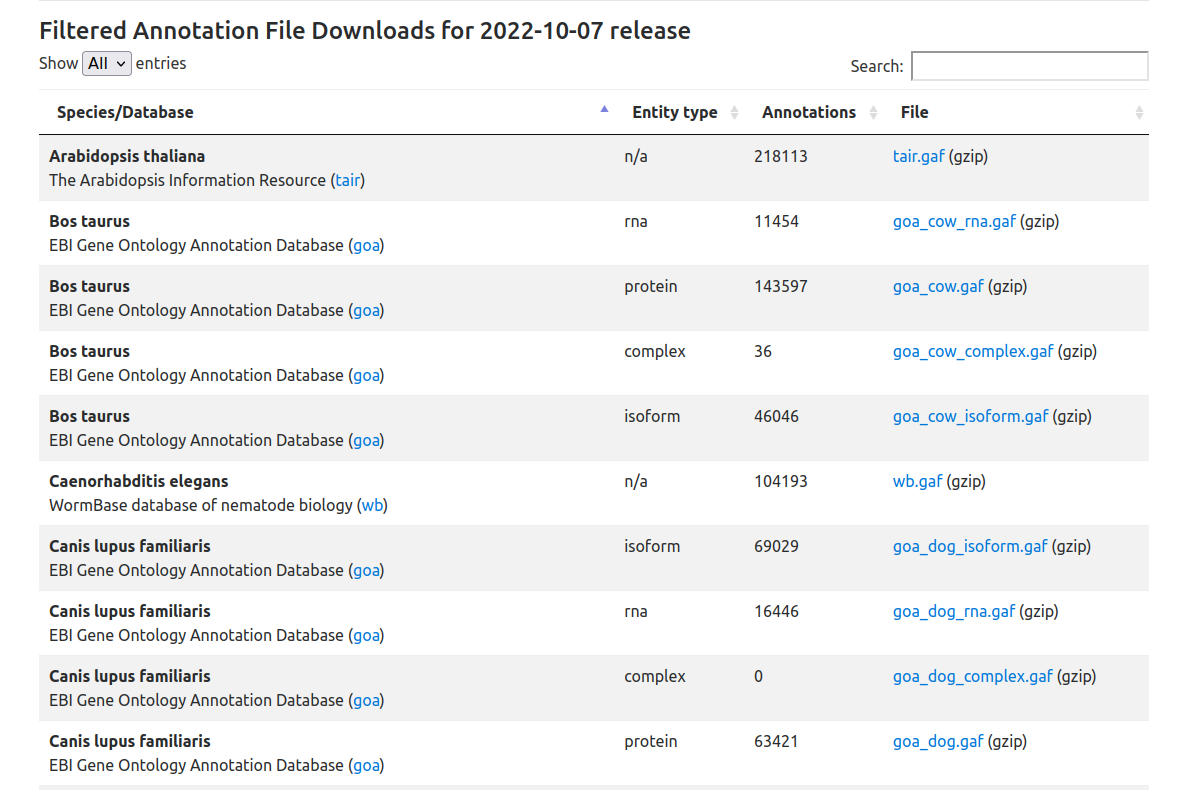
\includegraphics[width=0.7\textwidth]{img/go-gaf-page.png}
\end{center}
\begin{flushleft}
\begin{tiny}\textit{http://current.geneontology.org/products/pages/downloads.html}\end{tiny}
\end{flushleft}
\end{frame}

%%%%%%%%%%%%%%%%%%%%%%%%%%%%%%%%%%%%%%%%%%%%%%%
%%%%%%%%%%%%%%%%%%%%%%%%%%%%%%%%%%%%%%%%%%%%%%%

\begin{frame}{Example: fibrillin-1}
\begin{itemize}
\item Annotations are made for biological process, molecular function, and cellular component
\item evidence of source of the assertion (not shown)
\end{itemize} 

\begin{center}
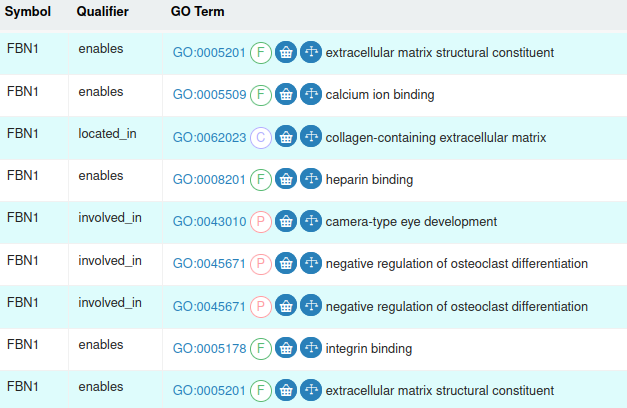
\includegraphics[width=0.7\textwidth]{img/fbn1-goa.png}
\end{center}
\end{frame}


%%%%%%%%%%%%%%%%%%%%%%%%%%%%%%%%%%%%%%%%%%%%%%%
%%%%%%%%%%%%%%%%%%%%%%%%%%%%%%%%%%%%%%%%%%%%%%%
\begin{frame}{GO: Overrepresentation Analysis}
\begin{mybluebox}{Question}
We have done a high throughput experiment and identified a list of differentially 
expressed genes. What are the salient characteristics of the genes in this list?
\end{mybluebox}

 \begin{itemize}
  \item We could just count the number of genes annotated to a certain GO term, but commomn things are common
  \item Instead, GO analysis asks the question of whether a given GO term is annotated {\bf more often than we would expect by chance}
\item Today, we will explain several algorithms for addressing this question. Similar approaches can be taken with other ontologies in a range of biological and medical settings.
 \end{itemize}

\end{frame}



%%%%%%%%%%%%%%%%%%%%%%%%%%%%%%%%%%%%%%%%%%%%%%%
%%%%%%%%%%%%%%%%%%%%%%%%%%%%%%%%%%%%%%%%%%%%%%%
\begin{frame}{binomial coefficient}
\begin{mybluebox}{Question?}
How do we calculate how many different sequences of outcomes there are if we flip a coin $n$ times?
\end{mybluebox}
\begin{columns}
\column{0.7\textwidth}
\begin{itemize}
\item  Each of the $n!$ rearrangements of the
numbers $1,2,\ldots,n$ defines a different rearrangement of the
letters $HHH\ldots HHTT\ldots TT$.
\item However, not all of the
rearrangements change the order of the $H$'s and the $T$'s. For
instance, exchanging the first two positions leaves the order
$HHH\ldots HHTT\ldots TT$ unchanged.
\end{itemize}
\column{0.3\textwidth}

\begin{center}
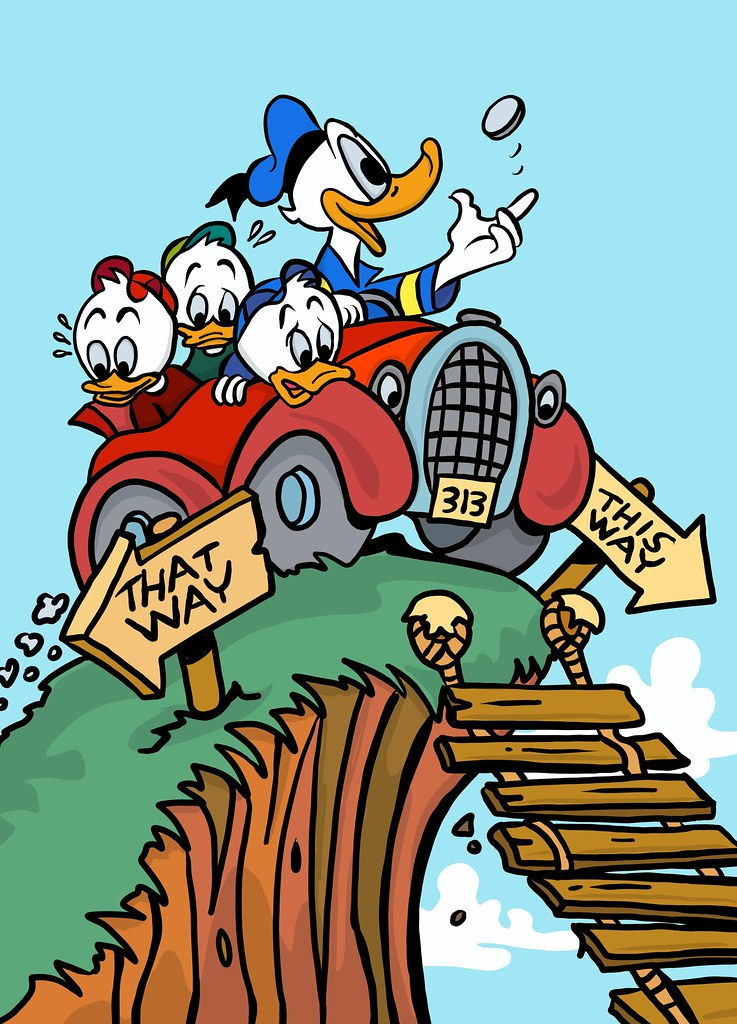
\includegraphics[width=1\textwidth]{img/donald.png}
\end{center}
\end{columns}

\end{frame}


%%%%%%%%%%%%%%%%%%%%%%%%%%%%%%%%%%%%%%%%%%%%%%%
%%%%%%%%%%%%%%%%%%%%%%%%%%%%%%%%%%%%%%%%%%%%%%%
\begin{frame}{binomial coefficient}

 \begin{mybluebox}{``$n$ choose $k$''}
The quantity $ \binom{n}{k} $ (read ``$n$ choose $k$'') is known as the binomial
coefficient.
\end{mybluebox}

 
\begin{itemize}
\item How do we calculate how many different sequences of outcomes there are if we flip a coin $n$ times?
\end{itemize}

  Noting that there are $k!$ ways of reordering the
``heads'' and $(n-k)!$ ways of reordering the ``tails,'' it follows
that there are
\begin{equation}
 \binom{n}{k} = \dfrac{n!}{\left(n-k\right)! k!}
\label{eq:binomial-coefficient}
\end{equation}
different ways of rearranging $k$ ``heads'' and $n-k$ ``tails.'' 

 
\end{frame}
%%%%%%%%%%%%%%%%%%%%%%%%%%%%%%%%%%%%%%%%%%%%%%%
%%%%%%%%%%%%%%%%%%%%%%%%%%%%%%%%%%%%%%%%%%%%%%%
\begin{frame}{binomial coefficient}
 \begin{mybluebox}{$k$ successes in $n$ attempts}
We are interested in the probability
of any one particular order of trials with $k$ successes and $n-k$
failures, we multiply the probabilities of the individual trials to
obtain $p^k(1-p)^{n-k}$. 
\end{mybluebox}

\begin{itemize}
\item We simply multiply the probability of one
particular trial order with $k$ successes and $n-k$ failures  by the number of trial
orders resulting in $k$ successes. 
\item This probability distribution is called the
\index{binomial distribution}
\textit{binomial distribution}:
\end{itemize}



\begin{equation}
 \label{eq:dbinomial}
P(k,n,p) = \binom{n}{k} p^k\left(1-p\right)^{n-k}
\end{equation} 
 
\end{frame}
%%%%%%%%%%%%%%%%%%%%%%%%%%%%%%%%%%%%%%%%%%%%%%%
%%%%%%%%%%%%%%%%%%%%%%%%%%%%%%%%%%%%%%%%%%%%%%%
\begin{frame}{binomial coefficient}


\begin{figure}[h!]
 \centering
 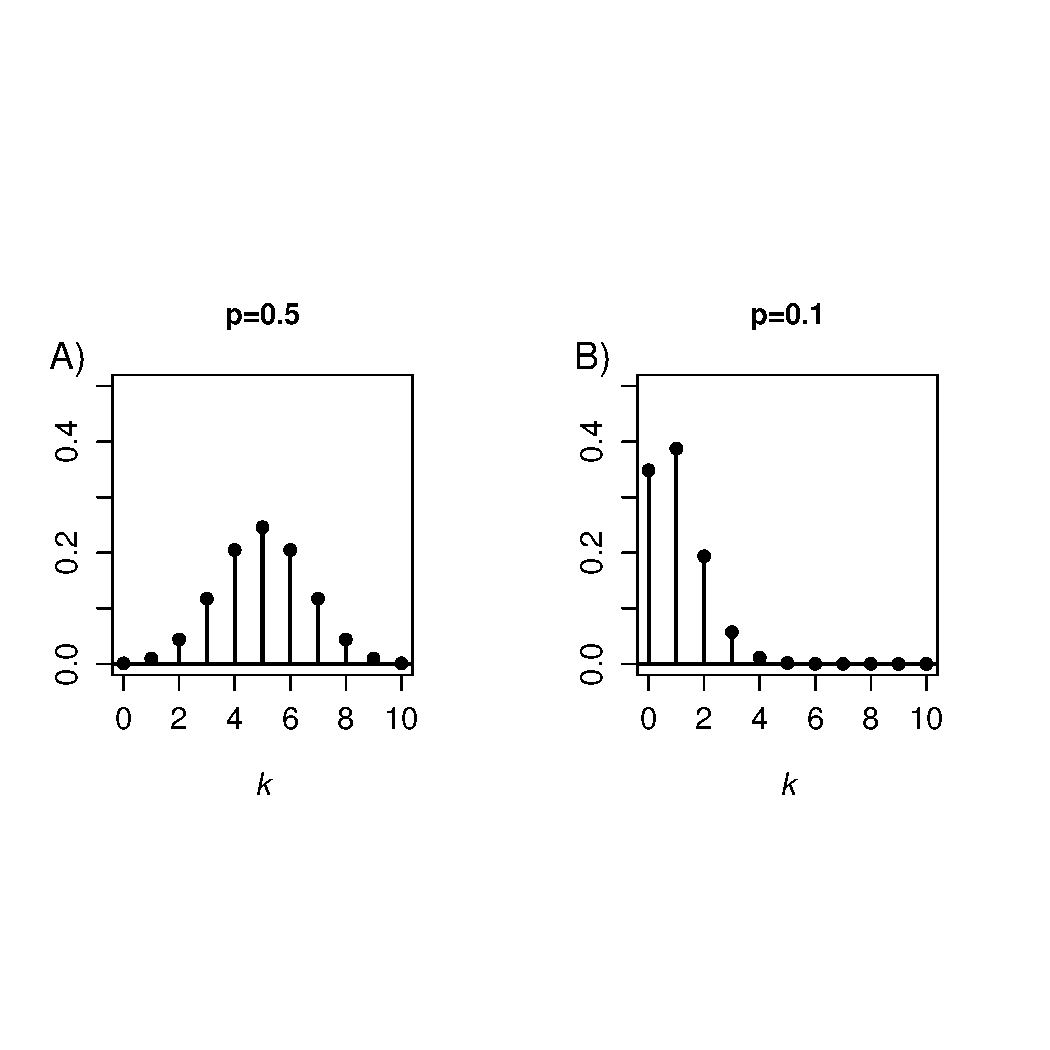
\includegraphics[width=.8\textwidth,viewport= 0 100 500 
380,clip]{img/binomial.pdf}
 \label{fig:binomial}
\end{figure}
\begin{description}
\item[A]the probability of
   $k=1,\ldots,10$ ``heads'' in ten coin tosses using a fair coin
   ($p=0.5$). 
   \item[B]Probability of $k=1,\ldots,10$ ``heads''
   in ten coin tosses using a biased coin ($p=0.1$).
\end{description} 
 
 

\end{frame}
%%%%%%%%%%%%%%%%%%%%%%%%%%%%%%%%%%%%%%%%%%%%%%%
%%%%%%%%%%%%%%%%%%%%%%%%%%%%%%%%%%%%%%%%%%%%%%%
\begin{frame}{GO Overrepresentation with the binomial distribution}
 \begin{mybluebox}{GO overrepresentation analysis}
each gene in the study set
is considered to be a ``trial,''  and ``success'' occurs if the gene is
annotated to a GO term of interest.
\end{mybluebox}
\begin{itemize}
\item The probability of ``success'' is simply the
frequency of the annotation to the GO term among all genes.  For
instance, if there are 10,000 genes are sequenced in an RNA-seq experiment, 600 of which
are annotated to some GO term $t$, then the probability of $t$ is
 $p=\frac{600}{10,000}=0.06$
\item If there are 250 differentially expressed genes, 30 of which are annotated to $t$, we can approximate the probability of observing exactly 30 genes in
the DE set annotated to $t$ as
\end{itemize}
\begin{equation}
\mathrm{P}(30,250,0.06)=1.44\times 10^{-4}
\end{equation}

 
\end{frame}
%%%%%%%%%%%%%%%%%%%%%%%%%%%%%%%%%%%%%%%%%%%%%%%
%%%%%%%%%%%%%%%%%%%%%%%%%%%%%%%%%%%%%%%%%%%%%%%
\begin{frame}{GO Overrepresentation}
 \begin{mybluebox}{null hypothesis}
 In order to use this for a statistical test,
 we now define a \textit{null hypothesis} to be
that the biological function described by GO term $t$ is not
overrepresented among the differentially expressed genes
\end{mybluebox}


\begin{itemize}
 \item if we
symbolize the proportion of genes in the population and study set that
are annotated to the term as $\pi_p$ and $\pi_s$, then
\end{itemize}
\begin{equation}
H_0:\pi_{s}\leq\pi_p 
\end{equation}

\end{frame}


%%%%%%%%%%%%%%%%%%%%%%%%%%%%%%%%%%%%%%%%%%%%%%%
%%%%%%%%%%%%%%%%%%%%%%%%%%%%%%%%%%%%%%%%%%%%%%%
\begin{frame}{GO Overrepresentation}
\begin{mybluebox}{alternative hypothesis}
Some GO term $t$ annotates a higher than expected proportion of the genes
in the study set.
\end{mybluebox}

\begin{equation}
H_A:\pi_{s}>\pi_p 
\end{equation}

\begin{itemize}
\item If the probability of the observed result of our experiment
(the observation of 30 genes in the DE set being annotated to $t$) is
less than $\alpha$, we reject the null hypothesis in favor of the
alternative hypothesis
\item This  would imply that the GO term $t$ has
something to do with the observed differential expression.
\end{itemize}


\end{frame}

%%%%%%%%%%%%%%%%%%%%%%%%%%%%%%%%%%%%%%%%%%%%%%%
%%%%%%%%%%%%%%%%%%%%%%%%%%%%%%%%%%%%%%%%%%%%%%%
\begin{frame}{GO Overrepresentation }
\begin{mybluebox}{Upper tail}
We calculate the probability of $\pi_{s}>\pi_p $ by calculating the probability of observing $k^{'}$ DE genes annotated to $t$ {\bf or more}, up to the maximum number of genes annotated to $t$ (because of only 100 gene are annotated to $t$, the probabilty of observing 101 or more is zero)
\end{mybluebox}

\begin{itemize}
\item  We take the sum to the maximum of the
number of genes annotated to a GO term $t$ (denoted $p_t$) or to the
size of the DE set (denoted $|\textit{DE}|$). 
\end{itemize}



\begin{equation}
 \label{eq:tailsumdbinomial}
p(k \geq k^{'},n,p) = \sum_{k=k^{'}}^{\max(p_t,|\textit{DE}|)}\binom{n}{k} 
k^p\left(n-k\right)^{1-p}.
\end{equation}  
 
 
\end{frame}

%%%%%%%%%%%%%%%%%%%%%%%%%%%%%%%%%%%%%%%%%%%%%%%
%%%%%%%%%%%%%%%%%%%%%%%%%%%%%%%%%%%%%%%%%%%%%%%
\begin{frame}{binomial distribution: Example}
 \begin{figure}[h!]
 \centering
 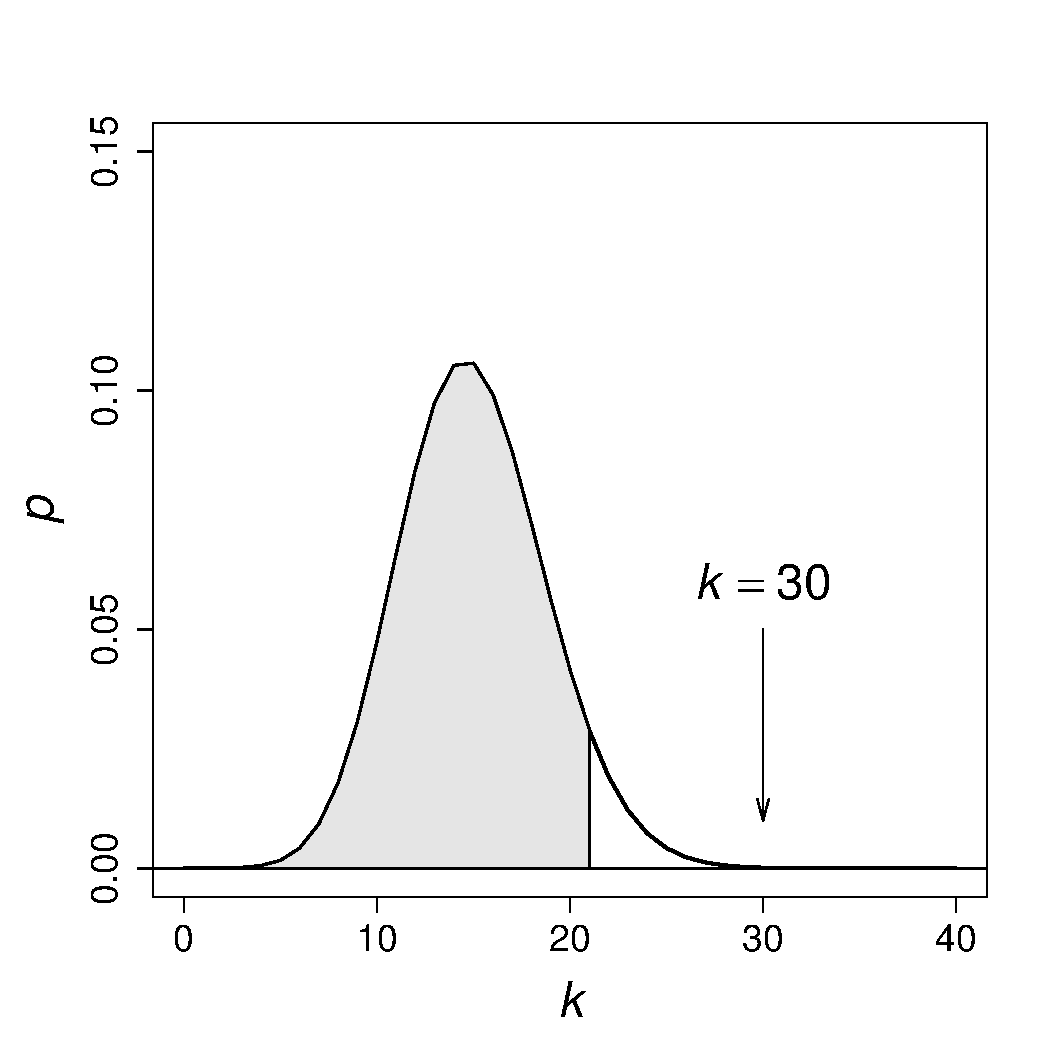
\includegraphics[width=0.4\textwidth]{img/Gobinom.pdf}
\end{figure}
\begin{scriptsize}Probability mass function (PMF)  with $p=0.06$ and
   $n=250$. Values for $k=0,1,\ldots,40$ are shown (the values for
   $k>40$ are nearly zero and are not shown). The observed value for
   $k$ of 30 lies outside of the range containing 95\% of the
   probability mass, and we reject the null hypothesis that the genes
   in the study set are not enriched in genes annotated by $t$. The
   $p$-value for this observation can be calculated by
   Equation~(\ref{eq:dbinomial}) to be $1.68\times 10^{-8}$.\end{scriptsize}
 
\end{frame}

%%%%%%%%%%%%%%%%%%%%%%%%%%%%%%%%%%%%%%%%%%%%%%%
%%%%%%%%%%%%%%%%%%%%%%%%%%%%%%%%%%%%%%%%%%%%%%%
\begin{frame}{binomial distribution: Example}
\begin{mybluebox}{To repalce or not to replace}
The individual tests are not independent if we do not replace drawn balls
\end{mybluebox}
\begin{figure}
\centering
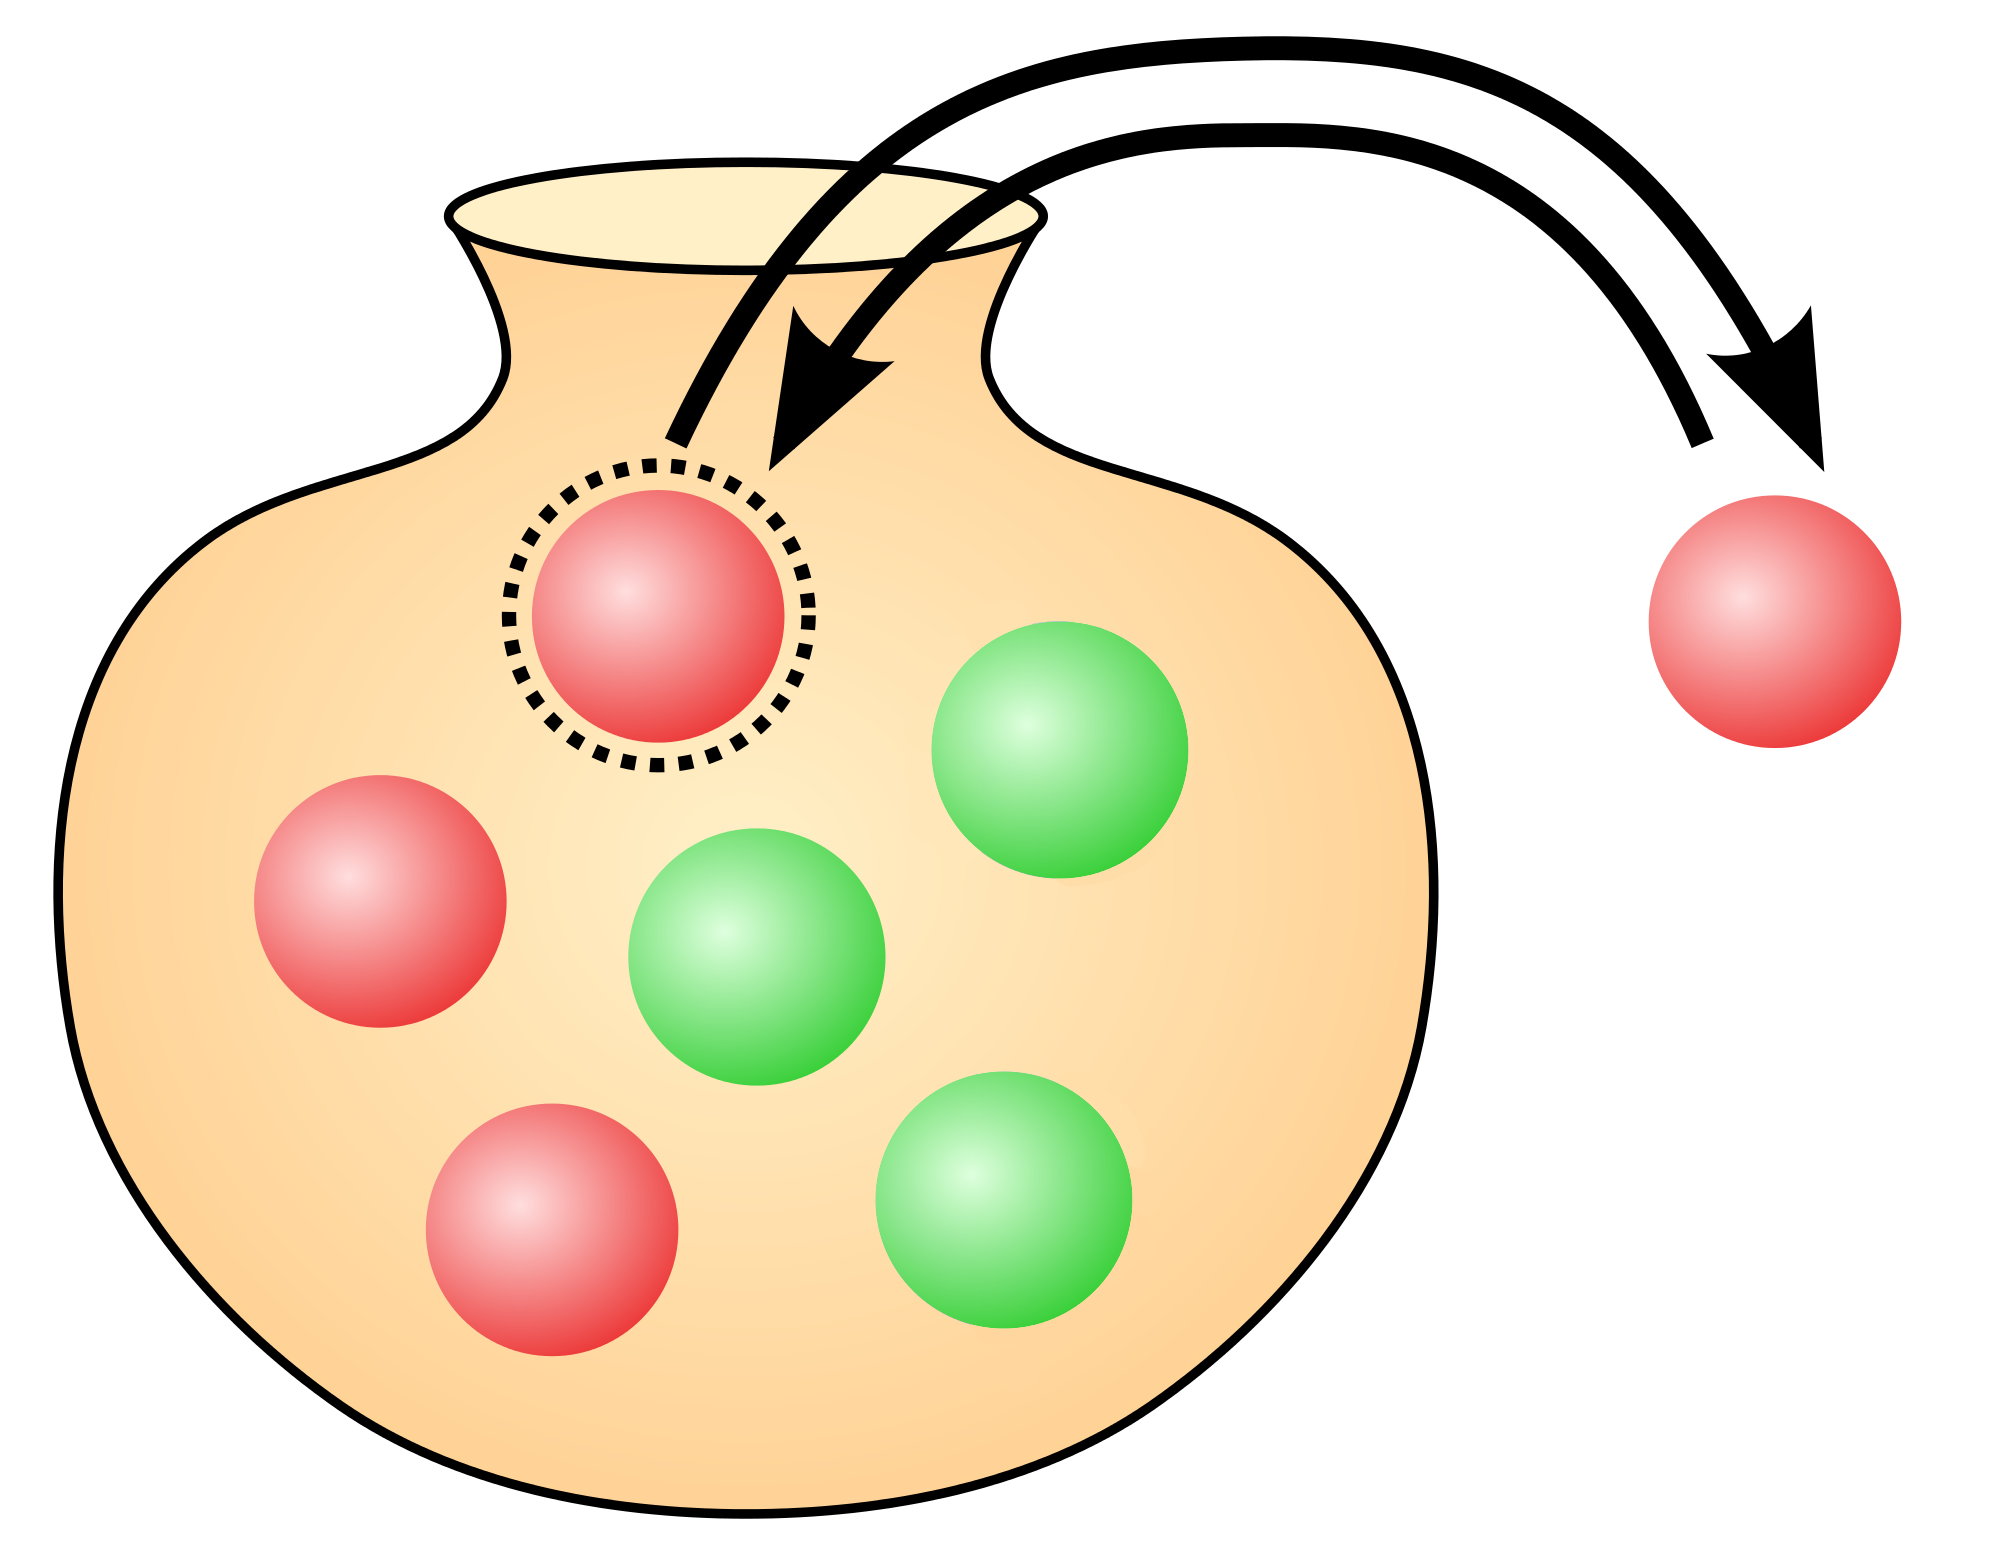
\includegraphics[width=0.4\textwidth]{img/urn.png} 

\end{figure}
\begin{itemize}
\item What is the probability of drawing a green ball if we replace the drawn red ball?
\item What is the probability  if we do not replace?

\end{itemize}

\end{frame}




%%%%%%%%%%%%%%%%%%%%%%%%%%%%%%%%%%%%%%%%%%%%%%%
%%%%%%%%%%%%%%%%%%%%%%%%%%%%%%%%%%%%%%%%%%%%%%%
\begin{frame}{binomial vs hypergeometric distribution}
\begin{mybluebox}{Faulty assumption}
 Although this approach provides a nearly correct answer for terms with
many annotations in the population and large DE sets, it is actually
only an approximation. 
\end{mybluebox}
\begin{itemize}
\item The problem is that the binomial distribution
is based on the assumption that the individual trials are independent
of one another. 
\item While this is clearly true for coin tosses, it is not
for GO overrepresentation analysis, which is rather comparable to a
lotto game in which labelled balls are taken from an urn and not
replaced.
\end{itemize}


\end{frame}



%%%%%%%%%%%%%%%%%%%%%%%%%%%%%%%%%%%%%%%%%%%%%%%
%%%%%%%%%%%%%%%%%%%%%%%%%%%%%%%%%%%%%%%%%%%%%%%

\begin{frame}{GO Overrepresentation with the hypergeometric distribution}
\begin{itemize}
\item In our
RNA-seq experiment, we imagine that the set of all 10,000 genes is represented by an urn with 10,000 balls.
\item  A total of 100 genes are
annotated to some GO term $t$, and thus 100 balls in the urn are
colored blue.
\item We then model the observation of 250 differentially
expressed genes as the process of randomly removing 250 balls in turn
from the urn without replacement. 
\end{itemize}
   
\end{frame}


%%%%%%%%%%%%%%%%%%%%%%%%%%%%%%%%%%%%%%%%%%%%%%%
%%%%%%%%%%%%%%%%%%%%%%%%%%%%%%%%%%%%%%%%%%%%%%%
\begin{frame}{Hypergeometric distribution}
\begin{mybluebox}{Approach}
count up all the ways of getting $k$ genes annotated to $t$ and $n-k$
remaining genes not annotated to $t$, and compare this number to the
number of all possible outcomes. 
\end{mybluebox}

\begin{tabular}{ll}
$m$ & total number of genes\\
$m_t$ & number of those genes that are annotated to GO term $t$\\
$n$ & number of DE genes (study set) \\
$k$& the number of DE genes that are annotated to $t$\\
\end{tabular}

\vspace{4mm}

\begin{equation}
 \label{eq:hypergeometric}
p(k,n,p)  = \dfrac{\binom{m_t}{k}\binom{m-m_t}{n-k}}{\binom{m}{n}}.
\end{equation}
\end{frame}



%%%%%%%%%%%%%%%%%%%%%%%%%%%%%%%%%%%%%%%%%%%%%%%
%%%%%%%%%%%%%%%%%%%%%%%%%%%%%%%%%%%%%%%%%%%%%%%
\begin{frame}{GO Overrepresentation with the hypergeometric distribution}
\begin{mybluebox}{Probability of exactly $m_t$ annotated genes in study set}
 \begin{equation}
p(k,n,p)  = \dfrac{\binom{m_t}{k}\binom{m-m_t}{n-k}}{\binom{m}{n}}.
\end{equation}
\end{mybluebox}

\begin{itemize}
 \item There are $\binom{m_t}{k}$ ways of
choosing $k$ genes annotated to $t$.
\item There are $\binom{m-m_t}{n-k}$
ways of choosing the remaining $n-k$ genes that are not annotated to
$t$.
\item   In total, there are $\binom{m_t}{k}\binom{m-m_t}{n-k}$ ways of
choosing the genes in the study set such that $k$ are annotated to $t$
and $n-k$ are not. 
\item There are $\binom{m}{n}$ total ways of choosing a
study set with $n$ genes from the population of $m$ genes with
arbitrary annotations.
\end{itemize}


 
\end{frame}

%%%%%%%%%%%%%%%%%%%%%%%%%%%%%%%%%%%%%%%%%%%%%%%%%%%%%%%%%%%%%%%%%%%%%%%%%%%%%%%%%%%%%%%%%%%%%%%%%%%
%%%%%%%%%%%%%%%%%%%%%%%%%%%%%%%%%%%%%%%%%%%%%%%%%%%%%%%%%%%%%%%%%%%%%%%%%%%%%%%%%%%%%%%%%%%%%%%%%%%%
\begin{frame}{Fisher's exact test}
\begin{mybluebox}{Probability of at least $m_t$ annotated genes in study set}
Equation~(\ref{eq:hypergeometric}) is known as the \textit{hypergeometric
distribution}. Analogously to the situation with the binomial
distribution, we need to calculate the probability of observing  $k^{'}$ {\bf or more} genes annotated to $t$ in order to have a
statistical test. 
\end{mybluebox}
 \begin{itemize}
 \item The sum over the tail of the
hypergeometric distribution is known as the \textbf{Exact Fisher
  Test}:
 \end{itemize}

\index{exact Fisher test}
\begin{equation}
 \label{eq:exactFisher}
p(K\geq k^{'},n,p) = 
\sum_{k=k^{'}}^{\max(K,|DE|)}\dfrac{\binom{m_t}{k}\binom{m-m_t}{n-k}}{\binom{m}{n}}
\end{equation}
 
 
\end{frame}

%%%%%%%%%%%%%%%%%%%%%%%%%%%%%%%%%%%%%%%%%%%%%%%%%%%%%%%%%%%%%%%%%%%%%%%%%%%%%%%%%%%%%%%%%%%%%%%%%%%
%%%%%%%%%%%%%%%%%%%%%%%%%%%%%%%%%%%%%%%%%%%%%%%%%%%%%%%%%%%%%%%%%%%%%%%%%%%%%%%%%%%%%%%%%%%%%%%%%%%%
\begin{frame}{Fisher's exact test}

 we refer to the set of genes which are investigated in an experiment as the
\emph{population set}. Note that we use the term \emph{gene} only for
simplicity. The items annotated to the ontology terms may also be proteins or
other biological entities. 

\begin{itemize}
 \item We denote this set by the uppercase letter $M$,
while the cardinality of the population set is denoted by $m$.
\item  If, for example,
a microarray experiment is conducted, the population set will comprise all genes
that the microarray chip can detect. The outcome of the experiment is referred
to as the \emph{study set}. It is denoted by $N$ and has the cardinality $n$.
\item 
 In
the microarray or RNA-seq scenario the study set could consist of all genes that were
detected to be differentially expressed.
\end{itemize}

\end{frame}

%%%%%%%%%%%%%%%%%%%%%%%%%%%%%%%%%%%%%%%%%%%%%%%%%%%%%%%%%%%%%%%%%%%%%%%%%%%%%%%%%%%%%%%%%%%%%%%%%%%
%%%%%%%%%%%%%%%%%%%%%%%%%%%%%%%%%%%%%%%%%%%%%%%%%%%%%%%%%%%%%%%%%%%%%%%%%%%%%%%%%%%%%%%%%%%%%%%%%%%%
\begin{frame}{Term-for-Term}
 The standard approach to identify the most interesting terms is to
perform Fisher's exact test for each term separately. For this reason,
we refer to this procedure as the term-for-term (TfT)
approach

\begin{itemize}
 \item For each GO term $t$, the genes in the population set $M$ are either
annotated to term $t$ or not.
\item This divides the population set into two
classes of items, comparable to an urn with white and
black marbles. 
\item We denote the set of all genes in the population that
are annotated to GO term $t$ as  $M_t$ and the cardinality of the set
as $m_t$.
\end{itemize}

 
\end{frame}
%%%%%%%%%%%%%%%%%%%%%%%%%%%%%%%%%%%%%%%%%%%%%%%%%%%%%%%%%%%%%%%%%%%%%%%%%%%%%%%%%%%%%%%%%%%%%%%%%%%
%%%%%%%%%%%%%%%%%%%%%%%%%%%%%%%%%%%%%%%%%%%%%%%%%%%%%%%%%%%%%%%%%%%%%%%%%%%%%%%%%%%%%%%%%%%%%%%%%%%%
\begin{frame}{Term-for-Term}
\begin{mybluebox}{study set}
 The study set is assumed to be a random sample that is
obtained by drawing $n$ genes without replacement
\end{mybluebox}
 \begin{itemize}
 \item The random variable that describes the number of genes of
the study set that are annotated to $t$ in this random sample, denoted
by $X_t$, therefore follows the \index{hypergeometric distribution}
hypergeometric distribution, i.e.,
 \end{itemize}



\begin{equation}
X_t \sim h(k|m;m_t;n) := P(X_t=k) = \frac{\displaystyle{m_t \choose
    k}\displaystyle{{m - m_t} 
\choose {n - k}}}{\displaystyle{m \choose n}}.
\label{eq:hypergeometric-term-for-term}
\end{equation}
\begin{tiny}
 $P(X_t=k)$ gives the probability of observing exactly $k$
annotated genes in a study set of size $n$ if the population set of
size $m$ contains $m_t$ genes that are annotated to term $t$.
\end{tiny}
\end{frame}
%%%%%%%%%%%%%%%%%%%%%%%%%%%%%%%%%%%%%%%%%%%%%%%%%%%%%%%%%%%%%%%%%%%%%%%%%%%%%%%%%%%%%%%%%%%%%%%%%%%
%%%%%%%%%%%%%%%%%%%%%%%%%%%%%%%%%%%%%%%%%%%%%%%%%%%%%%%%%%%%%%%%%%%%%%%%%%%%%%%%%%%%%%%%%%%%%%%%%%%%
\begin{frame}{Term-for-Term}
% \begin{displaybox}
%  Null and alternative hypothesis
% \end{displaybox}

 The
 number of genes in the study
set that are annotated to $t$ represents the observation. This number
is denoted by $n_t$. Now we want to assess whether the study set is
enriched for term $t$, i.e., whether the observed $n_t$ is higher than
one would expect. In order to formulate a statistical test, we need to
formulate a null hypothesis ($H_0$) and an alternative hypothesis
($H_1$). 
\begin{itemize}
 \item The null hypothesis in this case simply states that there is
no positive association between genes annotated to the term $t$ and
the study set; that is, there is no overrepresentation of term
$t$.
\item The alternative hypothesis is that there is overrepresentation of
the term.
\end{itemize}

\end{frame}


%%%%%%%%%%%%%%%%%%%%%%%%%%%%%%%%%%%%%%%%%%%%%%%%%%%%%%%%%%%%%%%%%%%%%%%%%%%%%%%%%%%%%%%%%%%%%%%%%%%
%%%%%%%%%%%%%%%%%%%%%%%%%%%%%%%%%%%%%%%%%%%%%%%%%%%%%%%%%%%%%%%%%%%%%%%%%%%%%%%%%%%%%%%%%%%%%%%%%%%%
\begin{frame}{Term-for-Term}
 
The null hypothesis
corresponds to the probability of observing a test statistic that is at least as
extreme as the one that was observed given that the null hypothesis is true.
\begin{itemize}
 \item Therefore, the null
hypothesis corresponding to a one-sided
test is rejected if the probability of observing $n_t$ \textit{or more} genes
annotated to term $t$ in the study set by chance is less than
$\alpha$ 
\item By convention, $\alpha$ is usually set to 0.05
\end{itemize}

  This is given by:

\begin{equation}
  P(X_t\geq n_t|H_0) = \sum_{k=n_t}^{\min(m_t,n)} 
 \frac{\displaystyle{m_t \choose k}\displaystyle{{m - m_t} 
 \choose {n - k}}}{\displaystyle{m \choose n}}.
\label{eqn:fisher.tft}
\end{equation}

 
\end{frame}
%%%%%%%%%%%%%%%%%%%%%%%%%%%%%%%%%%%%%%%%%%%%%%%%%%%%%%%%%%%%%%%%%%%%%%%%%%%%%%%%%%%%%%%%%%%%%%%%%%%
%%%%%%%%%%%%%%%%%%%%%%%%%%%%%%%%%%%%%%%%%%%%%%%%%%%%%%%%%%%%%%%%%%%%%%%%%%%%%%%%%%%%%%%%%%%%%%%%%%%%
\begin{frame}{Term-for-Term}

  Interpretation of ``significant'' GO terms

\begin{itemize}
 \item if $P(X_t\geq n_t|H_0) < \alpha$, the null hypothesis is
rejected, and we declare the term $t$ to be \textit{significantly
overrepresented} in the study set.
\item The biological interpretation of
significant overrepresentation is usually taken to be that the term
$t$ represents an important biological characteristic of the study
set.
\end{itemize}

 
 
\end{frame}
\begin{frame}


\begin{itemize}
 \item  Suppose that there is a population set of $m=18$ genes, of which
  $m_t=4$ genes are annotated to the term $t$.
  \item The outcome of an
  experiment conducted on all 18 genes of the population yields a set
  of 5 genes. This means that the study set consists of $n=5$
  genes.
  \item Moreover, we observe that a total of $n_t=3$ genes from the
  genes of the study set are annotated to term
  $t$ 
\end{itemize}


  We would now like to analyze whether term $t$ is significantly
  overrepresented in the study set and thus can be interpreted to
  represent an important result of the experiment:
\[
P(X_t\geq 3|H_0) = \frac{\displaystyle{5 \choose 3}\displaystyle{{13} \choose {2}}}{\displaystyle{18 
\choose 5}} + \frac{\displaystyle{5 \choose 4}\displaystyle{{13} \choose {1}}}{\displaystyle{18 
\choose 5}}
   = 0.044.
\]
\begin{tiny}Since $P(X_t\geq 3|H_0)=0.044<0.05=\alpha$, the null-hypotheses is
rejected and the term may be interpreted as being characteristic of
the experiment.\end{tiny}

\end{frame}

%------------------------------------------------


%------------------------------------------------


%------------------------------------------------



%----------------------------------------------------------------------------------------
%	 SECTION 2
%----------------------------------------------------------------------------------------

\section{Section 2}

%------------------------------------------------
\end{document}
\begin{frame}{Blocks}
	These blocks are part of 1 slide, to be displayed consecutively.
	\begin{block}{Block}
		Text.
	\end{block}
	\pause % Automatically creates a new "page" split between the above and above + below
	\begin{alertblock}{Alert block}
		Alert \alert{text}.
	\end{alertblock}
	\pause % Automatically creates a new "page" split between the above and above + below
	\begin{exampleblock}{Example block}
		Example \textcolor{example}{text}.
	\end{exampleblock}
\end{frame}


%----------------------------------------------------------------------------------------
%	 CLOSING/SUPPLEMENTARY SLIDES
%----------------------------------------------------------------------------------------

\appendix

\begin{frame}{References}
	\nocite{*} % Display all references regardless of if they were cited
	\bibliography{semalgs.bib}
	\bibliographystyle{plain}
\end{frame}

%------------------------------------------------

\begin{frame}{Backup Slide}
	This is a backup slide, useful to include additional materials to answer questions from the audience.
	\vfill
	The package \texttt{appendixnumberbeamer} is used to refrain from numbering appendix slides.
\end{frame}

%----------------------------------------------------------------------------------------

\end{document}
